\section{Options disponibles}
\subsection{Afficher la version}
\label{optionversion}

Par défaut, le numéro de version n'est pas affiché sur la première de couverture, comme sur le modèle Word. Cependant, cette information peut être intéressante et une option du \textit{package} permet de le faire. \\

Pour cela, il suffit de préciser l'option \texttt{version} et d'instancier la macro correspondante.

\begin{latex}
\usepackage[version]{telecom}
[...]
\version{1.2.3}
[...]
\begin{document}
\end{latex}

\subsection{Choix du campus}
\label{optioncampus}

Sur la dernière de couverture est affichée l'adresse. Par défaut, il s'agit de l'adresse du campus de Brest, cependant, les options \texttt{Rennes} et \texttt{Toulouse} permettent d'afficher l'adresse du campus correspondant. \\
Noter que l'option \texttt{Brest} existe mais est optionnelle.\\

\begin{minipage}[c]{0.6\textwidth}
\begin{latex}
\usepackage{telecom}
% ou \usepackage[Brest]{telecom}
\end{latex}
\end{minipage}
\vrule\begin{minipage}[c]{0.4\textwidth}
\centering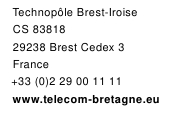
\includegraphics{brest}
\end{minipage}\\

\begin{minipage}[c]{0.6\textwidth}
\begin{latex}
\usepackage[Rennes]{telecom}
\end{latex}
\end{minipage}
\vrule\begin{minipage}[c]{0.4\textwidth}
\centering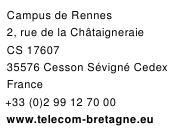
\includegraphics{rennes}
\end{minipage}\\

\begin{minipage}[c]{0.6\textwidth}
\begin{latex}
\usepackage[Toulouse]{telecom}
\end{latex}
\end{minipage}
\vrule\begin{minipage}[c]{0.4\textwidth}
\centering
\includegraphics{toulouse}
\end{minipage}\\
